\documentclass[12pt,letterpaper]{exam}
\usepackage[lmargin=1in,rmargin=1in,tmargin=1in,bmargin=1in]{geometry}
\usepackage{../style/exams}

% -------------------
% Course & Exam Information
% -------------------
\newcommand{\course}{MATH 115: Exam 3}
\newcommand{\term}{Fall --- 2024}
\newcommand{\examdate}{11/21/2024}
\newcommand{\timelimit}{50 Minutes}

\setbool{hideans}{false} % Student: True; Instructor: False

% -------------------
% Content
% -------------------
\begin{document}

\examtitle
\instructions{Write your name on the appropriate line on the exam cover sheet. This exam contains \numpages\ pages (including this cover page) and \numquestions\ questions. Check that you have every page of the exam. Answer the questions in the spaces provided on the question sheets. Be sure to answer every part of each question and show all your work. If you run out of room for an answer, continue on the back of the page --- being sure to indicate the problem number.} 
\scores
\bottomline
\newpage


% -------------------
% Questions
% -------------------
\begin{questions}

% Question 1
\newpage
\question[15] Compute the exact value for the following: \par\vspace{0.3cm}
	\begin{enumerate}[(a)]
	\item $\sin(240^\circ)= -\sin(60^\circ)= -\dfrac{\sqrt{3}}{2}$ \vfill
	\item $\csc \!\left( \dfrac{2\pi}{3} \right)= \dfrac{1}{\sin\left( \dfrac{2\pi}{3} \right)}= \dfrac{1}{\sin \left( \dfrac{\pi}{3} \right)}= \dfrac{2}{\sqrt{3}}$ \vfill
	\item $\tan \!\left(\dfrac{3 \pi}{2} \right)= \text{undefined}$ \vfill
	\item $\sec(135^\circ)= \dfrac{1}{\cos(135^\circ)}= \dfrac{1}{-\cos(45^\circ)}= -\sqrt{2}$ \vfill
	\item $\cos(\pi)= -1$ \vfill
	\end{enumerate}



% Question 2
\newpage
\question[15] Compute the exact value for the following: \par\vspace{0.3cm}
	\begin{enumerate}[(a)]
	\item $\sin^{-1} \!\!\left( -\dfrac{1}{2} \right)= -\dfrac{\pi}{6}$ \vfill
	\item $\arccos \!\left( \dfrac{1}{\sqrt{2}} \right)= \dfrac{\pi}{4}$ \vfill
	\item $\tan^{-1}(-1)= -\dfrac{\pi}{4}$ \vfill
	\item $\arccos \!\left( \dfrac{\sqrt{3}}{2} \right)= \dfrac{\pi}{6}$ \vfill
	\item $\arctan(-\infty)= -\dfrac{\pi}{2}$ \vfill
	\end{enumerate}



% Question 3
\newpage
\question[10] For each part below, give a trigonometric identity as described in the problem statement.
	\begin{enumerate}[(a)]
	\item Write $\cos(2x)$ in terms of \textit{both} $\sin(x)$ and $\cos(x)$. \vfill
		\[
		\cos(2x)= \cos^2(x) - \sin^2(x)
		\] \vfill
	\item Write $\tan^2(x)$ in terms of \textit{only} $\sec(x)$. \vfill
		\[
		\tan^2(x)= \sec^2(x) - 1
		\] \vfill
	\item Write an identity for $\tan(A \pm B)$. \vfill
		\[
		\tan(A \pm B)= \dfrac{\tan A \pm \tan B}{1 \mp \tan A \tan B}
		\] \vfill
	\item Write an identity for $\sin(A \pm B)$. \vfill
		\[
		\sin(A \pm B)= \sin A \cos B \pm \sin B \cos A
		\] \vfill
	\end{enumerate}



% Question 4
\newpage
\question[20] Showing all your work, answer the following problems: \par\vspace{0.1cm}
	\begin{enumerate}[(a)]
	\item Compute $\sin \!\big( \!\arctan(-4) \big)$ 

	{\itshape If $\theta= \arctan(-4)$, then $\tan \theta= -4 < 0$ so $\theta$ is in Quadrant~II or IV. But we know that $\arctan y$ always returns an angle in $(-\frac{\pi}{2}, \frac{\pi}{2})$. Therefore, $\theta:= \arctan(-4)$ is an angle in Quadrant~IV. Using the fact that $\tan \theta= -4= -\frac{4}{1}$ and $\tan \theta= \frac{\text{opp}}{\text{adj}}$, we have the following diagram:
		\[
		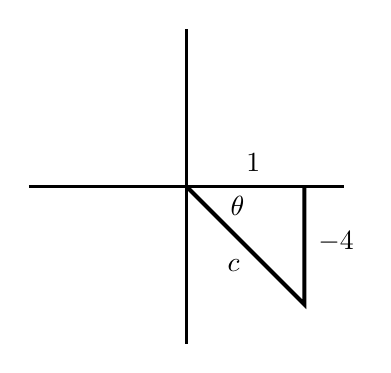
\begin{tikzpicture}
		\draw[line width=0.03cm] (-2,0) -- (2,0);
		\draw[line width=0.03cm] (0,-2) -- (0,2);
		\draw[line width=0.05cm] (0,0) -- (1.5,-1.5) -- (1.5,0);
		\node at (0.65,-0.25) {$\theta$};
		\node at (0.85,0.3) {$1$};
		\node at (1.9,-0.7) {$-4$};
		\node at (0.6,-1.0) {$c$};
		\end{tikzpicture}
		\]
	By the Pythagorean Theorem, we know that $c^2= 1^2 + (-4)^2= 1 + 16= 17$. But then $c= \sqrt{17}$. Because $\sin \theta= \frac{\text{opp}}{\text{hyp}}$, we know that $\sin \theta= \dfrac{-4}{\sqrt{17}}$.
		\[
		\boxed{\sin \!\big(\!\arctan(-4) \big)= -\dfrac{4}{\sqrt{17}}}
		\]
	}
	
	\item If $\tan \theta= -\frac{5}{12}$ and $\cos \theta > 0$, compute $\sin(2 \theta)$. \par\vspace{0.1cm}
	
	{\itshape Because $\tan \theta= -\frac{5}{12} < 0$, we know that $\theta$ lies in Quadrant~II or IV. Because $\cos \theta > 0$, we know that $\theta$ lies in Quadrant~I or IV. Therefore, $\theta$ lies in Quadrant~IV. Using this fact, $\tan= -\frac{5}{12}$, and the fact that $\tan \theta= \frac{\text{opp}}{\text{adj}}$, we have the following picture:
		\[
		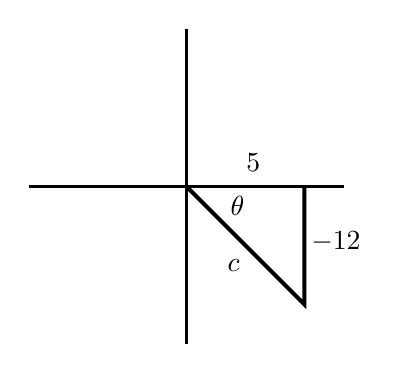
\begin{tikzpicture}
		\draw[line width=0.03cm] (-2,0) -- (2,0);
		\draw[line width=0.03cm] (0,-2) -- (0,2);
		\draw[line width=0.05cm] (0,0) -- (1.5,-1.5) -- (1.5,0);
		\node at (0.65,-0.25) {$\theta$};
		\node at (0.85,0.3) {$5$};
		\node at (1.9,-0.7) {$-12$};
		\node at (0.6,-1.0) {$c$};
		\end{tikzpicture}
		\]
	Using the Pythagorean Theorem, we know that $c^2= 5^2 + (-12)^2= 25 + 144= 169$. Therefore, $c= \sqrt{169}= 13$. Using the fact that $\sin(2\theta)= 2 \sin \theta \cos \theta$, $\sin \theta= \frac{\text{opp}}{\text{hyp}}$, and $\cos \theta= \frac{\text{adj}}{\text{hyp}}$, we have\dots
		\[
		\begin{gathered}
		\sin(2\theta)= 2 \sin \theta \cos \theta= 2 \cdot \dfrac{-12}{13} \cdot \dfrac{5}{13}= \dfrac{2 \cdot -60}{13^2}= -\dfrac{120}{169} \\[0.3cm]
		\boxed{\sin(2\theta)= -\dfrac{120}{169}}
		\end{gathered}
		\]
	}
	
	\end{enumerate}



% Question 5
\newpage
\question[10] Using the fact that $\dfrac{17\pi}{12}= \dfrac{5\pi}{3} - \dfrac{\pi}{4}$ and showing all your work, compute $\cos \left( \dfrac{17\pi}{12} \right)$. \pspace

{\itshape \tsol Using the difference-angle identity for $\cos$, we have\dots
	\[
	\begin{aligned}
	\cos \left( \dfrac{17\pi}{12} \right)&= \cos \left( \dfrac{5\pi}{3} - \dfrac{\pi}{4} \right) \\[0.3cm]
	&= \cos \left( \dfrac{5\pi}{3} \right) \cos \left( \dfrac{\pi}{4} \right) + \sin \left( \dfrac{5\pi}{3} \right) \sin \left( \dfrac{\pi}{4} \right) \\[0.3cm]
	&= \dfrac{1}{2} \cdot \dfrac{1}{\sqrt{2}} + \left( - \dfrac{\sqrt{3}}{2} \right) \cdot \dfrac{1}{\sqrt{2}} \\[0.3cm]
	&= \dfrac{1}{2 \sqrt{2}} - \dfrac{\sqrt{3}}{2 \sqrt{2}} \\[0.3cm]
	&= \dfrac{1 - \sqrt{3}}{2 \sqrt{2}}
	\end{aligned}
	\] \vfill

{\footnotesize Alternatively, although the instructions indicate that one must use the given composition of $\frac{17\pi}{12}$, one could use the half-angle identity of partial credit. Note that $\frac{17\pi}{12}$ is an angle in Quadrant~III, where $\cos \theta < 0$. But then\dots
	\[
	\begin{aligned}
	\cos \left( \dfrac{17\pi}{12} \right)&= \cos \left(\dfrac{1}{2} \cdot \dfrac{17\pi}{6} \right) \\
	&= -\sqrt{\dfrac{1 + \cos \left( \frac{17\pi}{6} \right)}{2}} \\
	&= -\sqrt{\dfrac{1 + \cos \left(2\pi + \frac{5\pi}{6} \right)}{2}} \\
	&= -\sqrt{\dfrac{1 + \cos \left(\frac{5\pi}{6} \right)}{2}} \\
	&= -\sqrt{\dfrac{1 - \frac{\sqrt{3}}{2}}{2}} \\
	&= -\sqrt{\dfrac{1 - \frac{\sqrt{3}}{2}}{2} \cdot \dfrac{2}{2}} \\
	&= -\sqrt{\dfrac{2 - \sqrt{3}}{4}}
	\end{aligned}
	\]
To see this is equivalent to the answer above, observe\dots
	\[
	-\sqrt{\dfrac{2 - \sqrt{3}}{4}}= -\sqrt{\dfrac{2 - \sqrt{3}}{4} \cdot \dfrac{2}{2}}= -\sqrt{\dfrac{4 - 2\sqrt{3}}{8}}= -\sqrt{\dfrac{(\sqrt{3} - 1)^2}{8}}= - \dfrac{\sqrt{3} - 1}{\sqrt{8}}= \dfrac{1 - \sqrt{3}}{2 \sqrt{2}}
	\]
     }
}



% Question 6
\newpage
\question[15] Find the value of $x$ in the triangle shown below. Be sure to show all your work.
	\[
	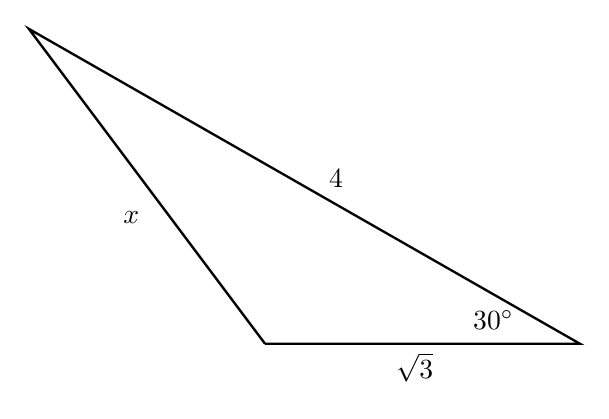
\begin{tikzpicture}
	\draw[line width=0.03cm] (0,0) -- (-3,4) -- (4,0) -- (0,0);
	\node at (-1.7,1.6) {$x$};
	\node at (1.9,-0.3) {$\sqrt{3}$};
	\node at (0.9,2.1) {$4$};
	\node at (2.9,0.3) {$30^\circ$};
	\end{tikzpicture}
	\] \pspace

{\itshape \tsol Using the law of cosines, we have\dots
	\[
	\begin{gathered}
	b^2= a^2 + c^2 - 2ac \cos B \\[0.3cm]
	x^2= (\sqrt{3})^2 + 4^2 - 2(\sqrt{3}) 4 \cos(30^\circ) \\[0.3cm]
	x^2= 3 + 16 - 8 \sqrt{3} \cos(30^\circ) \\[0.3cm]
	x^2= 19 - 8 \sqrt{3} \cdot \dfrac{\sqrt{3}}{2} \\[0.3cm] 
	x^2= 19 - 4(3) \\[0.3cm]
	x^2= 19 - 12 \\[0.3cm]
	x^2= 7 \\[0.3cm]
	x= \pm \sqrt{7} \\[0.3cm]
	x= \sqrt{7}
	\end{gathered}
	\]
Note. The last step follows because $x$ is a length and thusly $x \geq 0$.
}



% Question 7
\newpage
\question[15] Showing all your work, find all the exact solutions to the equation shown below. 
	\[
	8 \sin^2(2 \pi x - \pi) + 5= 9
	\] \pspace

\sol We have\dots
	\[
	\begin{gathered}
	8 \sin^2(2 \pi x - \pi) + 5= 9 \\[0.1cm]
	8 \sin^2(2 \pi x - \pi)= 4 \\[0.1cm]
	\sin^2(2 \pi x - \pi)= \dfrac{1}{2} \\[0.1cm]
	\sqrt{\sin^2(2 \pi x - \pi)}= \sqrt{\dfrac{1}{2}} \\[0.1cm]
	\sin(2\pi x - \pi)= \pm \dfrac{1}{\sqrt{2}}
	\end{gathered}
	\]
But then, there are four possibilities:
	
	\begin{center} \underline{\phantom{XXX}$\mathbf{x= \dfrac{1}{\sqrt{2}}}$\phantom{XXX}} \end{center}
	
	\[
	\begin{gathered}
	2\pi x - \pi= \dfrac{\pi}{4} \pm 2 \pi n \\[0.1cm]
	2\pi x= \dfrac{5\pi}{4} \pm 2 \pi n \\[0.1cm]
	\boxed{x= \dfrac{5}{8} \pm n}
	\end{gathered}
	\qquad \text{ OR } \qquad
	\begin{gathered}
	2\pi x - \pi= \dfrac{3\pi}{4} \pm 2 \pi n \\[0.1cm]
	2\pi x= \dfrac{7\pi}{4} \pm 2 \pi n \\[0.1cm]
	\boxed{x= \dfrac{7}{8} \pm n}
	\end{gathered}
	\]
	
	\begin{center} \underline{\phantom{XXX}$\mathbf{x= -\dfrac{1}{\sqrt{2}}}$\phantom{XXX}} \end{center}

	\[
	\begin{gathered}
	2\pi x - \pi= \dfrac{5\pi}{4} \pm 2 \pi n \\[0.1cm]
	2\pi x= \dfrac{9\pi}{4} \pm 2 \pi n \\[0.1cm]
	2\pi x= \dfrac{\pi}{4} + \dfrac{8\pi}{4} \pm 2 \pi n \\[0.1cm]
	2\pi x= \dfrac{\pi}{4} + 2\pi \pm 2 \pi n \\[0.1cm]
	2\pi x= \dfrac{\pi}{4} \pm 2 \pi n \\[0.1cm]
	\boxed{x= \dfrac{1}{8} \pm n}
	\end{gathered}
	\qquad \text{ OR } \qquad
	\begin{gathered}
	2\pi x - \pi= \dfrac{7\pi}{4} \pm 2 \pi n \\[0.1cm]
	2\pi x= \dfrac{11\pi}{4} \pm 2 \pi n \\[0.1cm]
	2\pi x= \dfrac{3\pi}{4} + \dfrac{8\pi}{4} \pm 2 \pi n \\[0.1cm]
	2\pi x= \dfrac{3\pi}{4} + 2\pi \pm 2 \pi n \\[0.1cm]
	2\pi x= \dfrac{3\pi}{4} \pm 2 \pi n \\[0.1cm]
	\boxed{x= \dfrac{3}{8} \pm n} \\[0.1cm]
	\end{gathered}
	\]
where $n$ is any integer. 

\end{questions}
\end{document}